\chapter{Background e Stato dell'Arte}

L'evoluzione del panorama delle minacce informatiche ha reso indispensabile lo sviluppo di tecniche e strumenti sempre più sofisticati per l'analisi forense digitale. Questo capitolo fornisce le basi teoriche necessarie per comprendere il contesto in cui si inserisce il presente lavoro, esplorando i concetti fondamentali del Digital Forensics and Incident Response (DFIR), con particolare attenzione all'analisi della memoria volatile. Verranno inoltre esaminati i principali framework esistenti. Infine, verrà illustrato cosa è YARA e quali sono i suoi principali utilizzi nell'ambito dell'analisi forense e della rilevazione di minacce.

\section{Digital Forensics e Incident Response (DFIR)}

\subsection{Definizione e principi fondamentali}

Il Digital Forensics and Incident Response (DFIR) rappresenta la convergenza di due discipline complementari che, insieme, formano il nucleo delle capacità di risposta alle minacce cyber moderne. Il termine DFIR è stato coniato per riflettere la natura interconnessa di queste attività nel contesto operativo reale.\\

La \textbf{Digital Forensics} è definita dal NIST come "l'applicazione di scienza e metodi per identificare, preservare, raccogliere, validare, analizzare, interpretare, documentare e presentare evidenze digitali derivate da fonti digitali allo scopo di facilitare o promuovere la ricostruzione di eventi" \cite{kent2006}. Questa disciplina si basa su quattro principi scientifici fondamentali:

\begin{itemize}
    \item \textbf{Preservazione dell'evidenza}: Garantire che i dati non vengano alterati durante l'acquisizione e l'analisi
    \item \textbf{Chain of custody}: Documentare ogni passaggio per mantenere l'ammissibilità legale
    \item \textbf{Ripetibilità}: Le analisi devono produrre risultati consistenti quando ripetute
    \item \textbf{Documentazione completa}: Ogni azione deve essere registrata e giustificata
\end{itemize}

Questi principi sono ulteriormente codificati negli standard internazionali come ISO/IEC 27037:2012 \cite{iso27037}, che fornisce linee guida per l'identificazione, raccolta, acquisizione e preservazione delle evidenze digitali. Lo standard enfatizza quattro principi cardine: rilevanza, affidabilità, sufficienza e conformità alle normative locali. Similmente, le linee guida SWGDE \cite{swgde2022} per l'acquisizione di contenuti online stabiliscono best practices specifiche per la preservazione di evidenze volatili come pagine web, social media e comunicazioni cloud-based.\\

L'\textbf{Incident Response}, d'altra parte, si concentra sulla gestione operativa degli incidenti di sicurezza con l'obiettivo di minimizzare l'impatto e ripristinare le operazioni normali nel minor tempo possibile. Il SANS Institute definisce l'IR come "un approccio organizzato per affrontare e gestire le conseguenze di una violazione della sicurezza o di un attacco informatico" \cite{sans2023}.\\

La fusione di queste discipline nel DFIR riconosce che, nel mondo reale, l'analisi forense e la risposta agli incidenti sono attività inseparabili. Durante un incidente attivo, i responder devono bilanciare molteplici esigenze contrastanti: contenere la minaccia mentre preservano le evidenze, analizzare i sistemi compromessi senza interrompere le operazioni critiche, e trovare il giusto equilibrio tra la necessità di un'indagine approfondita e l'urgenza del ripristino operativo.

\subsection{Fasi del processo DFIR}

Il processo DFIR segue un approccio metodologico articolato in sei fasi distinte, come definito dal framework NIST SP 800-61 \cite{cichonski2012}. Sebbene questa struttura fornisca un modello logico di riferimento, nella pratica operativa le fasi si sovrappongono frequentemente e richiedono un approccio iterativo, dove l'analisi forense permea trasversalmente l'intero processo fornendo le informazioni necessarie per decisioni informate in ogni momento.

\begin{figure}[ht]
    \centering
    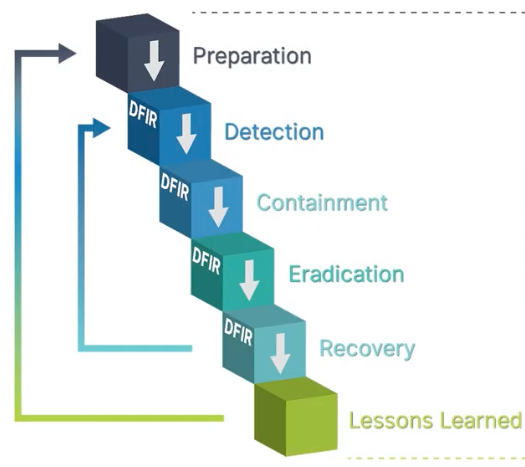
\includegraphics[width=0.6\linewidth]{images/stato-arte/digital-forensics-incident-response-plan-flow.png}
\end{figure}

\paragraph{1. Preparazione}
La preparazione rappresenta il fondamento dell'intero processo DFIR, determinando la differenza tra una risposta efficace in poche ore e una gestione caotica che può protrarsi per giorni. Questa fase richiede lo sviluppo preventivo di playbook e procedure operative standard per scenari ricorrenti, supportati da un'infrastruttura tecnologica adeguata. L'implementazione di meccanismi di logging pervasivi e la predisposizione di capacità di acquisizione forense immediatamente disponibili costituiscono prerequisiti essenziali. Parallelamente, il training continuo del personale attraverso simulazioni realistiche garantisce la prontezza operativa quando l'incidente si verifica.

\paragraph{2. Identificazione}
Il rilevamento tempestivo di un incidente può trasformare una potenziale catastrofe aziendale in un inconveniente gestibile. Questa fase inizia con l'analisi degli alert provenienti dai sistemi di sicurezza, seguita da un processo di triage che distingue i falsi positivi dalle minacce concrete. La determinazione accurata dello scope iniziale e della gravità potenziale permette l'attivazione mirata del team di risposta con le competenze specifiche richieste dalla situazione.

\paragraph{3. Contenimento}
Una volta confermato l'incidente, il contenimento diventa prioritario per limitare la propagazione del danno. L'approccio si articola su due livelli temporali complementari: le azioni immediate di contenimento a breve termine, come l'isolamento dei sistemi compromessi, e le misure sostenibili a lungo termine, che includono l'applicazione di patch temporanee mentre si prepara l'eradicazione definitiva. Cruciale in questa fase è l'acquisizione di backup forensi prima di qualsiasi modifica, accompagnata da una documentazione meticolosa per preservare la chain of custody.

\paragraph{4. Eradicazione}
L'eliminazione completa della minaccia richiede un approccio sistematico che va oltre la semplice rimozione degli artefatti visibili. L'identificazione di tutti i componenti malevoli, incluse backdoor e meccanismi di persistenza nascosti, deve essere seguita dalla chiusura definitiva delle vulnerabilità sfruttate. Il rafforzamento delle difese in questa fase non si limita alla remediation immediata, ma include misure preventive contro tecniche di attacco simili.

\paragraph{5. Recupero}
Il ripristino delle operazioni normali rappresenta una fase delicata dove la fretta può vanificare gli sforzi precedenti. La ricostruzione dei sistemi deve partire esclusivamente da backup verificati e puliti, accompagnata da un monitoraggio intensificato che si protrae per settimane. La validazione sistematica del ripristino delle funzionalità business-critical e l'implementazione di controlli compensativi temporanei assicurano la continuità operativa mentre si consolida la sicurezza dell'ambiente.

\paragraph{6. Lessons Learned}
La fase conclusiva, troppo spesso sacrificata alla pressione di considerare l'incidente "chiuso", rappresenta invece l'opportunità fondamentale per il miglioramento continuo. La documentazione dettagliata dell'intero evento e l'analisi critica della risposta permettono di identificare punti di forza e debolezza del processo. L'aggiornamento di procedure e playbook basato sull'esperienza acquisita, insieme alla condivisione responsabile di IOC e lessons learned con la community, trasforma ogni incidente in un'opportunità di crescita per l'organizzazione e per l'ecosistema di sicurezza nel suo complesso.

\subsection{Importanza nell'ambito della cybersecurity moderna}

Il DFIR è ormai un pilastro della cybersecurity, poiché le minacce attuali richiedono capacità avanzate e rispondono anche a stringenti obblighi normativi. Gli \textit{Advanced Persistent Threats (APT)} coinvolgono attori statali o sindacati criminali che mantengono accessi prolungati alle reti per esfiltrare dati, monetizzarli o ottenere vantaggi geopolitici. Il modello \textit{Ransomware-as-a-Service (RaaS)} ha democratizzato gli attacchi ransomware, consentendo anche a criminali poco esperti di lanciare campagne devastanti. Gli \textit{supply chain attacks}, come il caso SolarWinds \cite{solarwinds2020}, dimostrano come un singolo fornitore compromesso possa impattare migliaia di organizzazioni. Le tecniche di \textit{living-off-the-land} sfruttano strumenti legittimi già presenti nei sistemi (PowerShell, WMI, scheduled tasks), rendendo la detection molto più complessa.

Sul piano normativo, il GDPR \cite{gdpr2016} impone la notifica delle violazioni entro 72 ore, la direttiva NIS2 \cite{nis2_2022} estende tali obblighi a operatori essenziali e fornitori digitali, mentre il DORA \cite{dora2022} richiede capacità di incident response testate e validate nel settore finanziario. Parallelamente, il tempo medio di permanenza degli attaccanti è sceso a 16 giorni \cite{mandiant2023}, ma con differenze marcate: le organizzazioni con DFIR maturo rilevano intrusioni in pochi giorni, quelle meno preparate in mesi, aumentando i rischi di esfiltrazione, movimento laterale e persistenza.

Infine, il DFIR non è più solo reattivo: ogni incidente genera \textit{Threat Intelligence} (IOC, TTP, lezioni operative) che, se condivisa e analizzata, rafforza la postura difensiva e crea un ciclo virtuoso di miglioramento continuo.


\section{Memory Forensics}

\subsection{Concetti base della memoria volatile}

La memoria volatile, principalmente la RAM (Random Access Memory), rappresenta lo stato “vivo” di un sistema informatico in un preciso istante. A differenza dello storage persistente, che conserva i dati anche senza alimentazione, la memoria volatile ospita informazioni effimere ma fondamentali in ambito forense, poiché rivelano con precisione cosa stava accadendo al momento dell’acquisizione \cite{ligh2014}.

\subsubsection{Architettura della memoria}
L’architettura della memoria segue una gerarchia pensata per bilanciare velocità, capacità e costi. I registri della CPU sono rapidissimi (un ciclo di clock) ma con capacità minima, mentre le cache L1, L2 e L3 forniscono buffer sempre più ampi ma progressivamente più lenti. La RAM principale costituisce l’area di lavoro del sistema, accessibile in circa un centinaio di cicli, mentre le aree di memory-mapped I/O sono dedicate alla comunicazione diretta con i dispositivi hardware.

Dal punto di vista forense, la RAM principale rappresenta il target privilegiato, poiché offre la visione più completa dello stato del sistema. Al suo interno troviamo lo spazio kernel, che contiene le strutture critiche del sistema operativo, driver e tabelle di sistema; lo spazio utente, dove risiedono processi, librerie e dati applicativi; la pool memory, utilizzata dal kernel per allocazioni dinamiche; e la page cache, che conserva temporaneamente i dati dei file recentemente utilizzati.

\subsubsection{Gestione della memoria virtuale}
La gestione della memoria virtuale nei sistemi operativi moderni introduce ulteriore complessità ma anche opportunità investigative. Ogni processo viene isolato dagli altri attraverso uno spazio di indirizzamento dedicato, che gli fornisce l’illusione di avere l’intera memoria a disposizione. In realtà, le pagine virtuali sono mappate dinamicamente su frame fisici, mentre il paging consente di spostare su disco (pagefile o swap) le pagine meno utilizzate per liberare RAM.

Per l’analista forense, ricostruire correttamente la memoria virtuale a partire dal dump fisico significa saper navigare strutture come page tables, translation lookaside buffers (TLB) e memory descriptors. Queste strutture, sebbene complesse, sono anche prevedibili e quindi sfruttabili per ottenere una rappresentazione fedele dello stato dei processi al momento dell’acquisizione.

\subsection{Tipologie di artefatti recuperabili}

La memoria volatile conserva una varietà di artefatti che non esistono altrove o che su disco risultano cifrati \cite{case2017}. La loro analisi fornisce un quadro unico e difficilmente replicabile con altre fonti di evidenza.

Un primo insieme di artefatti riguarda \textbf{processi e thread}. È possibile recuperare la lista completa dei processi, inclusi quelli nascosti da rootkit sofisticati, e analizzare argomenti della command line, variabili d’ambiente, handle aperti verso file o oggetti kernel, stack e heap contenenti informazioni utili alla ricostruzione dell’esecuzione, fino ai moduli e alle DLL caricati, che possono essere verificati in termini di integrità.

Accanto a questi, le \textbf{informazioni di rete} presenti in memoria offrono uno snapshot delle comunicazioni in corso. Si possono individuare connessioni TCP/UDP attive con indirizzi e porte, socket in ascolto che potrebbero nascondere backdoor, raw socket usati per sniffing o attacchi, oltre a cache DNS, routing table, ARP cache e buffer di pacchetti non ancora elaborati.

La memoria custodisce anche numerosi \textbf{artefatti di sicurezza}. Qui risiedono, in forma decifrata e temporanea, token di autenticazione, chiavi di cifratura di volumi protetti (BitLocker, FileVault, TrueCrypt), certificati e chiavi di sessione SSL/TLS, ticket Kerberos, hash NTLM utilizzabili per attacchi pass-the-hash e persino password di applicazioni rese momentaneamente disponibili durante l’uso.

Un’altra categoria cruciale è costituita dalle \textbf{evidenze di malware}. Malware sofisticati possono esistere esclusivamente in RAM: codice iniettato in processi legittimi, API hooks, driver kernel malevoli, payload cifrati che vengono decifrati solo al momento dell’esecuzione, buffer di comunicazioni Command \& Control e shellcode in corso di esecuzione. In molti casi, queste tracce sono assenti dal disco e recuperabili unicamente in memoria.

Non meno rilevanti sono le \textbf{tracce di attività utente}. La clipboard può contenere dati sensibili copiati, mentre titoli e contenuti parziali di finestre aperte, cronologia dei comandi di shell non ancora persistita, documenti in fase di modifica, form data e credenziali web temporaneamente memorizzati, così come chat e messaggi in chiaro, offrono spunti preziosi per ricostruire il comportamento dell’utente.

Infine, la memoria conserva \textbf{metadati di sistema} che arricchiscono il contesto investigativo: registry hives caricati, log di eventi non ancora flushati su disco, dati di prefetch, record di ShimCache e AmCache, metadati delle shadow copies e cache del file system, tutti elementi che permettono una timeline forense più accurata.

\subsection{Vantaggi rispetto all'analisi tradizionale del disco}

L’analisi della memoria offre vantaggi unici, spesso superiori a quella del disco. Innanzitutto garantisce \textbf{visibilità su minacce avanzate}: malware fileless, reflective DLL injection, process hollowing e l’abuso di strumenti legittimi (PowerShell, WMI, scheduled tasks) sfuggono all’analisi statica dei file.

Consente inoltre l’\textbf{accesso a dati cifrati}: database, documenti protetti e comunicazioni SSL/TLS possono essere osservati in chiaro durante l’esecuzione, e le chiavi di full-disk encryption devono risiedere in RAM per funzionare.

La memoria offre una \textbf{visione runtime completa}: processi in esecuzione, oggetti di sincronizzazione, connessioni di rete temporanee e allocazioni dinamiche non ricostruibili dal disco, insieme a una \textbf{timeline più accurata}, difficilmente falsificabile rispetto ai timestamp del file system.

Dal punto di vista metodologico, l’analisi della memoria rispetta gli \textbf{standard forensi}. La norma ISO/IEC 27037 \cite{iso27037} riconosce la memoria volatile come fonte critica di evidenza, mentre le linee guida SWGDE \cite{swgde2022} indicano procedure specifiche di acquisizione, semplificando la chain of custody grazie al dump unico prodotto.

Infine, questa tecnica permette di \textbf{bypassare molte contromisure anti-forensi}: la modifica dei file o la cancellazione sicura non influiscono sulle strutture in RAM, e rootkit o strumenti di cifratura lasciano tracce inevitabili durante l’esecuzione.

\section{Volatility 3 Framework}

Volatility \cite{volatility2024} rappresenta indiscutibilmente il gold standard nell'analisi forense della memoria, evolvendosi da progetto sperimentale a framework di riferimento mondiale per la community DFIR. La sua storia è una testimonianza dell'importanza dell'open source nella sicurezza informatica.

\subsubsection{Storia ed evoluzione}
Il percorso di Volatility inizia nel 2007 quando Aaron Walters, frustrato dalla mancanza di tool accessibili per l'analisi della memoria, rilascia Volatility 1.0. Questo rilascio rivoluziona il campo, democratizzando l'accesso a tecniche precedentemente riservate a poche agenzie governative e aziende con tool proprietari costosi.

Nel 2011, Volatility 2.0 introduce un'architettura plugin-based che trasforma il framework da tool monolitico a piattaforma estensibile. Questa decisione architettonica si rivela geniale, permettendo alla community di contribuire con centinaia di plugin specializzati per ogni tipo di analisi immaginabile.

Il 2019 segna una svolta con Volatility 3, una riscrittura completa in Python 3 che risolve limitazioni architetturali accumulate negli anni. La nuova versione introduce un sistema di simboli più flessibile, migliore gestione della memoria e performance significativamente migliorate. Nel 2024, Volatility supporta le ultimissime versioni di Windows 11, Linux kernel 6.x e sta espandendo il supporto per architetture ARM e Apple Silicon.

\subsubsection{Architettura di Volatility 3}
L'eleganza di Volatility 3 risiede nella sua architettura modulare ed estensibile:

Il \textbf{Framework Core} orchestra tutti i componenti, gestendo configurazione, logging, e flusso di esecuzione. Fornisce API consistenti che nascondono la complessità sottostante ai plugin developers.

Le \textbf{Symbol Tables} costituiscono il cuore della capacità di Volatility di interpretare strutture di dati raw in memoria. Ogni versione di ogni sistema operativo ha strutture leggermente diverse, e Volatility mantiene un database comprensivo di questi "simboli" per interpretare correttamente i dati.

Gli \textbf{Address Spaces} forniscono un'astrazione elegante per accedere a diversi formati di dump di memoria. Che si tratti di un raw dump, un crash dump di Windows, o un formato proprietario di un hypervisor, l'address space appropriato traduce gli accessi in modo trasparente.

I \textbf{Plugins} implementano la logica specifica per estrarre artefatti particolari. Ogni plugin è specializzato in un aspetto dell'analisi: processi, rete, registry, malware detection, etc.

I \textbf{Renderers} gestiscono l'output, permettendo risultati in formato human-readable, JSON per automazione, CSV per analisi in Excel, o formati custom per integrazione con altri tool.

\subsubsection{Capacità principali}
Volatility 3 offre un arsenale impressionante di oltre 100 plugin che coprono virtualmente ogni aspetto dell'analisi forense.\\
Per l'analisi dei processi, plugin fondamentali includono:
\begin{itemize}
    \item \textbf{pslist/pstree}: Visualizzano processi in lista o albero gerarchico
    \item \textbf{psscan}: Trova processi nascosti scannerizzando la memoria
    \item \textbf{cmdline}: Estrae command line complete con tutti gli argomenti
    \item \textbf{dlllist}: Enumera tutte le DLL caricate da ogni processo
    \item \textbf{handles}: Lista tutti gli handle aperti (file, registry, mutex, etc.)
\end{itemize}
L'analisi di rete è coperta da:
\begin{itemize}
    \item \textbf{netscan}: Scanner comprensivo per Windows Vista+
    \item \textbf{netstat}: Per sistemi legacy Windows XP/2003
    \item \textbf{connections/sockets}: Per sistemi Linux
\end{itemize}
La detection di malware include plugin sofisticati:
\begin{itemize}
    \item \textbf{malfind}: Identifica code injection e modifiche sospette
    \item \textbf{hollowfind}: Rileva process hollowing
    \item \textbf{callbacks}: Enumera callback kernel spesso abusati da rootkit
    \item \textbf{ssdt}: Verifica integrità della System Service Descriptor Table
\end{itemize}

\subsubsection{Vantaggi di Volatility 3}
Il successo duraturo di Volatility deriva da vantaggi fondamentali difficili da replicare. La natura open source con licenza permissiva ha creato una community di contributori da università, aziende e agenzie governative worldwide. L'estensibilità attraverso plugin permette a chiunque di aggiungere funzionalità specializzate senza modificare il core. Il supporto per dozzine di formati di dump diversi lo rende universalmente applicabile. La documentazione estensiva e i training disponibili abbassano la barriera all'ingresso. Infine, anni di uso in casi reali hanno stabilito Volatility come tool forensicamente valido e legalmente accettabile in tribunale.

\subsubsection{Limitazioni}
Nonostante la sua potenza, Volatility presenta limitazioni significative che ne impediscono l'adozione più ampia. L'interfaccia command-line, per quanto potente per gli esperti, risulta intimidatoria per utenti meno tecnici. Interpretare correttamente l'output richiede una profonda conoscenza delle strutture del sistema operativo - sapere che un processo ha certi handle aperti è inutile se non si comprende cosa questo implichi. L'output testuale richiede un significativo post-processing per creare visualizzazioni o report comprensibili. Non esiste automazione built-in per workflow comuni, costringendo a scripting manuale. Infine, la mancanza di gestione integrata di casi multipli rende difficile organizzare investigazioni complesse che coinvolgono dozzine di sistemi.

\subsection{Limitazioni degli approcci attuali}

Nonostante la maturità e varietà degli strumenti disponibili, l'adozione della memory forensics rimane limitata rispetto al suo potenziale. Le limitazioni sistemiche creano barriere che scoraggiano molte organizzazioni dall'investire in questa capacità critica.

\subsubsection{Barriera tecnica elevata}
La complessità tecnica richiesta rimane il principale ostacolo all'adozione. Non si tratta solo di imparare comandi - l'analisi efficace richiede comprensione profonda di come i sistemi operativi gestiscono memoria, processi, driver e sottosistemi. Interpretare correttamente i risultati richiede esperienza per distinguere comportamenti normali da anomalie. Anche task apparentemente semplici come "trova processi sospetti" richiedono conoscenza di cosa costituisca "sospetto" in contesti diversi. La necessità di scripting per qualsiasi automazione esclude ulteriormente personale non programmatore.

\subsubsection{Mancanza di standardizzazione}
L'industria non ha raggiunto consenso su standard comuni, risultando in:
\begin{itemize}
    \item Formati di output incompatibili tra tool diversi
    \item Impossibilità di condividere facilmente risultati tra team che usano tool diversi  
    \item Ogni integrazione SIEM/SOAR richiede sviluppo custom
    \item Workflow e procedure che variano drasticamente tra organizzazioni
    \item Difficoltà nel creare training standardizzato
\end{itemize}

\subsubsection{Scalabilità limitata}
I tool esistenti sono progettati per analisi di singoli dump, creando colli di bottiglia in scenari reali:
\begin{itemize}
    \item Incidenti enterprise possono coinvolgere centinaia di endpoint
    \item Analisi sequenziale di dump multipli richiede tempo proibitivo
    \item Mancanza di parallelizzazione nativa forza workaround manuali
    \item Storage di dump multipli (100GB+ ciascuno) diventa rapidamente problematico
    \item Correlazione tra findings di sistemi diversi è manuale e error-prone
\end{itemize}

\subsubsection{User experience inadeguata}
L'esperienza utente non ha tenuto il passo con le aspettative moderne:
\begin{itemize}
    \item Output testuale denso scoraggia utenti abituati a dashboard interattive
    \item Mancanza di visualizzazioni rende difficile vedere pattern e relazioni
    \item Navigare migliaia di righe di output richiede pazienza infinita
    \item Generare report comprensibili per management richiede ore di lavoro manuale
    \item Collaborazione tra team members è complicata da formati proprietari
\end{itemize}

\subsubsection{Integrazione limitata}
L'isolamento dei tool di memory forensics dal resto dell'ecosistema di sicurezza limita il loro valore:
\begin{itemize}
    \item Threat intelligence feeds non si integrano nativamente
    \item Correlazione con logs, network traffic, e altri data source è manuale
    \item Export verso piattaforme di analisi avanzata richiede trasformazioni complesse
    \item API limitate o assenti impediscono automazione enterprise
    \item Mancanza di connettori per piattaforme SOAR moderne
\end{itemize}

Queste limitazioni non sono mere inconvenienze - creano un gap sostanziale tra il valore teorico della memory forensics e la sua applicazione pratica quotidiana. In contesti ad alta pressione come incident response real-time o cyber defense exercises, queste inefficienze possono fare la differenza tra successo e fallimento.

\section{YARA: Pattern Matching nella Memory Forensics}

\subsection{Introduzione a YARA}

YARA, acronimo ricorsivo per "Yet Another Recursive Acronym" \cite{yara2024}, è diventato lo standard per il pattern matching e la classificazione di malware nell'ambito della sicurezza informatica. Creato da Victor M. Alvarez presso VirusTotal nel 2008, YARA è nato dall'esigenza di fornire ai ricercatori di sicurezza uno strumento flessibile e potente per identificare e classificare campioni di malware basandosi su pattern testuali o binari.

Il concetto alla base di YARA è semplice: permettere la creazione di "regole" che descrivono famiglie di malware (o qualsiasi tipo di pattern) basandosi su caratteristiche testuali o binarie. Queste regole possono poi essere applicate a file, processi in memoria o dump di memoria per identificare rapidamente la presenza di minacce conosciute o comportamenti sospetti.

\subsection{Sintassi e struttura delle regole YARA}

Una regola YARA segue una struttura ben definita che bilancia espressività e semplicità:

\begin{minted}[
    breaklines,
    frame=lines,
    framesep=2mm,
    baselinestretch=1.2,
    fontsize=\small,
    linenos
]{xml}
rule ExampleRule {
    meta:
        author = "Security Researcher"
        description = "Detects Example Malware"
        date = "2024-01-01" 
    strings:
        $text_string = "malicious_function"
        $hex_string = { 6A 40 68 00 30 00 00 6A 14 8D }
        $regex = /\w+\.exe/
    condition:
        any of them
}
\end{minted}


Le regole YARA sono composte da tre sezioni principali:
\begin{itemize}
    \item \textbf{Meta}: Contiene metadati descrittivi sulla regola (autore, descrizione, riferimenti)
    \item \textbf{Strings}: Definisce i pattern da cercare (stringhe testuali, sequenze esadecimali, regex)
    \item \textbf{Condition}: Specifica la logica booleana per determinare quando una regola matcha
\end{itemize}

La potenza di YARA risiede nella sua flessibilità. Le condizioni possono essere semplici ("any of them") o estremamente complesse, utilizzando operatori logici, contatori, offset di memoria e funzioni built-in per creare logiche di detection sofisticate.

\subsection{YARA nell'analisi della memoria}

L'applicazione di YARA all'analisi della memoria rappresenta un'evoluzione naturale del suo utilizzo tradizionale su file statici. Quando applicato a dump di memoria, YARA diventa uno strumento potentissimo per:

\subsubsection{Identificazione di malware in memoria}
Molti malware moderni non lasciano tracce su disco e risiedono unicamente nella memoria RAM, dove vengono eseguiti dopo essere stati decifrati o decompressi in fase di runtime. In questo contesto, YARA si rivela particolarmente utile per identificare questi payload, che altrimenti sfuggirebbero a un'analisi basata sui file salvati:
\begin{itemize}
  \item Shellcode iniettato in processi legittimi
  \item DLL reflective caricate dinamicamente
  \item Payload di exploit dopo lo sfruttamento di vulnerabilità
\end{itemize}

\subsubsection{Hunting per indicatori di compromissione}
Durante un'indagine forense, è spesso necessario cercare indicatori di compromissione (IOC) all'interno della memoria per confermare o approfondire un sospetto di intrusione. Le YARA rules consentono di scandagliare la memoria alla ricerca di elementi distintivi legati a malware o attività malevole:
\begin{itemize}
  \item Stringhe uniche associate a famiglie di malware
  \item Pattern di comunicazione C2 (Command and Control)
  \item Artefatti di tool di post-exploitation
\end{itemize}

\subsubsection{Rilevamento di tecniche di evasione}
I malware più sofisticati impiegano tecniche avanzate per evitare il rilevamento, interferendo con i processi e le strutture di sistema. YARA può individuare pattern associati a queste tecniche, fornendo indizi preziosi per smascherare tentativi di elusione:
\begin{itemize}
  \item Process hollowing signatures
  \item Hook di API sospetti
  \item Modifiche a strutture critiche del kernel
\end{itemize}

\subsubsection{Analisi comportamentale}
Oltre al rilevamento basato su stringhe statiche, YARA può essere utilizzata per evidenziare comportamenti anomali in memoria, utili per classificare famiglie di malware o scoprire varianti sconosciute. Questo approccio permette una visione più dinamica dell'attacco:
\begin{itemize}
  \item Pattern di allocazione memoria anomali
  \item Sequenze di API call sospette
  \item Strutture dati associate a specifiche famiglie di malware
\end{itemize}

\subsection{Integrazione con Volatility}

Volatility include nativamente il plugin \texttt{yarascan}, che consente di applicare regole YARA direttamente a dump di memoria. Questa integrazione rende estremamente pratico cercare pattern sospetti senza dover estrarre manualmente porzioni di memoria o analizzare singoli processi uno alla volta.

Il plugin \texttt{yarascan} non si limita a segnalare i match trovati, ma restituisce anche un ricco contesto, fondamentale per l'analisi forense e per ricostruire in maniera accurata lo scenario di compromissione. In particolare, fornisce:
\begin{itemize}
  \item \textbf{Offset di memoria del match}, utile per correlare il dato con altre strutture o per esportare la regione di interesse.
  \item \textbf{Processo proprietario della memoria}, che permette di attribuire il dato rilevato a un particolare processo e capire se si tratta di un'attività lecita o sospetta.
  \item \textbf{Permessi della pagina di memoria} (ad esempio RWX), spesso indicativi di tecniche di iniezione o allocazioni anomale.
  \item \textbf{Dump del contenuto circostante}, che consente un'analisi manuale più approfondita, come la ricerca di stringhe, header binari o ulteriori indizi.
\end{itemize}
Queste informazioni contestuali trasformano un semplice match di pattern in un vero e proprio punto di partenza per ricostruire il comportamento del malware o identificare tecniche di evasione avanzate.


\subsection{Vantaggi di YARA per la memory forensics}

L'adozione di YARA nell'analisi della memoria offre numerosi benefici che ne fanno uno strumento fondamentale per i professionisti della digital forensics. Innanzitutto, YARA introduce un alto grado di standardizzazione: le sue regole forniscono un linguaggio comune e condiviso per descrivere pattern malevoli, facilitando lo scambio di intelligence tra team e organizzazioni diverse. Questo significa che una regola scritta da un analista può essere immediatamente applicata da un altro, senza bisogno di traduzioni o adattamenti complessi.

Un altro punto di forza è la notevole flessibilità. La sintassi di YARA permette di definire condizioni di detection anche molto articolate, mantenendo al contempo la leggibilità e la chiarezza del codice. Questo è cruciale quando si devono descrivere scenari complessi, che coinvolgono molteplici stringhe, byte pattern e relazioni logiche.

Sul piano delle prestazioni, il motore di YARA è progettato per essere estremamente efficiente, in grado di eseguire scansioni rapide anche su volumi significativi di dati. Questo lo rende adatto non solo ad analisi offline ma anche a contesti di monitoraggio in tempo reale.

Un ulteriore vantaggio è dato dalla manutenibilità. Le regole YARA sono semplici file di testo, facilmente versionabili e sottoponibili a peer review, il che consente una gestione strutturata dei rule set in repository condivisi. Infine, la portabilità delle regole rappresenta un valore aggiunto: la stessa regola può essere applicata a file su disco, dump di memoria o persino traffico di rete, massimizzando così il ritorno dell’investimento nello sviluppo delle detection logic.

\subsection{Limitazioni e sfide}

Nonostante i numerosi punti di forza, l’uso di YARA nella memory forensics non è privo di criticità e sfide operative. La prima riguarda la complessità intrinseca della memoria virtuale: a causa della frammentazione e della gestione a pagine, un pattern potrebbe risultare spezzato su più pagine non contigue, rendendo inefficace un approccio di matching puramente lineare.

Esiste poi il rischio di generare falsi positivi, specialmente quando si utilizzano pattern troppo generici che possono accidentalmente corrispondere a dati legittimi presenti in memoria. Questo problema si amplifica in un ambiente dove coesistono contemporaneamente moltissimi processi e tipi diversi di dati.

Va inoltre considerata la capacità di evasione dei malware più evoluti. Tecniche come la cifratura o l’offuscamento delle stringhe, la frammentazione intenzionale delle signature o l’uso del polimorfismo vengono adottate proprio per sfuggire a meccanismi di pattern matching statico come quelli di YARA.

Anche sul fronte delle performance, sebbene YARA sia molto ottimizzato, le scansioni di grandi dump di memoria possono richiedere tempi significativi, soprattutto quando si utilizzano rule set particolarmente estesi.

Infine, un efficace utilizzo di YARA presuppone una manutenzione continua delle regole. Le minacce evolvono costantemente e un rule set che oggi risulta efficace potrebbe diventare obsoleto nel giro di poche settimane o mesi. Questo implica la necessità di allocare risorse e definire processi strutturati per l’aggiornamento e la validazione delle regole stesse.


\subsection{YARA nell'ecosistema di sicurezza moderno}

YARA si è evoluto ben oltre il suo scopo originario di semplice motore di pattern matching per file su disco, diventando oggi un componente strategico nell'ecosistema di sicurezza informatica. Le piattaforme di threat intelligence, come MISP e OpenCTI, ad esempio, supportano nativamente le regole YARA come tipo di indicatore, consentendo così la distribuzione automatizzata di nuove detection attraverso reti di collaborazione tra analisti e organizzazioni. Questo rende estremamente rapido il passaggio dal rilevamento di una nuova minaccia alla protezione concreta delle infrastrutture.

Allo stesso modo, molte soluzioni EDR (Endpoint Detection and Response) integrano YARA per effettuare scansioni in tempo reale sui processi in esecuzione e sui file che vengono creati o modificati sui sistemi endpoint. Ciò permette di intercettare comportamenti malevoli direttamente alla fonte, riducendo i tempi di risposta agli incidenti.

Anche i sistemi di sandboxing, spesso utilizzati per l’analisi dinamica dei malware, impiegano YARA per classificare automaticamente i campioni analizzati, accelerando così le attività di triage e prioritizzazione. Parallelamente, i moderni SIEM e SOAR sfruttano le regole YARA per arricchire gli eventi di sicurezza con contesto aggiuntivo e per attivare playbook di risposta automatizzata, rendendo l'intero processo più efficiente.

Questa diffusione capillare di YARA in praticamente ogni segmento della sicurezza informatica ne fa oggi una competenza imprescindibile per qualunque professionista del settore. L'integrazione di YARA in strumenti di memory forensics rappresenta quindi non solo un potenziamento tecnico, ma una vera e propria evoluzione necessaria per mantenere efficacia e rilevanza in un panorama di minacce in continua trasformazione.